
\section{Placement}
\label{sec:placement}
So far we have only dealt with technology problems where we consider the problem space and adress the constraints of the hardware architecture. 
For every constraint, we devise a solution or a simplification to reduce the complexity of the problem space. 

Now that we have dealt with the bulk of these constraints and squared them away into self-contained \texttt{SiteInst}s, we can now apply some general optimization algorithms to finally address our optimization objective, which is to place these \texttt{SiteInst}s onto the device while minimizing wirelength. 

In this paper we implement and present a Simulating Annealing (SA) placer that operates at the \texttt{SiteInst} level. 



\subsection{Simulated Annealing}
\label{subsec:simulated_annealing}

\begin{lstlisting}[language=java, caption={Simulated Annealing pseudocode}, label={lst:sa_pseudocode}]
public void placeDesign(PackedDesign packedDesign) {
    // unplace the pseudorandom packed placement
    unplaceAllSiteInsts(packedDesign);
    // place randomly
    randomInitialPlacement(packedDesign);
    int moves = 0;
    while (moves < 300) {
        move(packedDesign)
        updateTemperature();
        moves++;
    }
}

private void move(PackedDesign packedDesign) {
    moveSiteChains(packedDesign.DSPSiteInstCascades);
    moveSiteChains(packedDesign.CARRYSiteInstChains);
    moveSingleSite(packedDesign.RAMSiteInsts);
    moveSingleSite(packedDesign.CLBSiteInsts);
}

protected void moveSingleSite(List<SiteInst> sites) {
    for (SiteInst si : sites) {
        // We refer to the current Site si as the "home site"
        // We refer to the proposed Site as the "away site"

        // Find the list of Sites connected to the home site
        List<Site> homeConns = findConnectedSites(si);

        Site homeSite = si.getSite();
        // Select an away site (random selection, midpoint, centroid, etc.)
        Site awaySite = proposeSite();

    }
}

protected void moveSingleSite(List<SiteInst> sites) {
    for (SiteInst si : sites) {
        SiteTypeEnum ste = si.getSiteTypeEnum();
        List<Site> homeConns = findConnectedSites(si, null);
        Site homeSite = si.getSite();
        Site awaySite = proposeSite(si, homeConns, true);
        SiteInst awaySi = occupiedSites.get(ste).get(awaySite);
        double oldCost = 0;
        double newCost = 0;
        if (awaySi != null) {
            List<Site> awayConns = findConnectedSites(awaySi, null);
            oldCost += evaluateSite(homeConns, homeSite);
            oldCost += evaluateSite(awayConns, awaySite);
            newCost += evaluateSite(homeConns, awaySite);
            newCost += evaluateSite(awayConns, homeSite);
        } else {
            oldCost += evaluateSite(homeConns, homeSite);
            newCost += evaluateSite(homeConns, awaySite);
        }
        if (evaluateMoveAcceptance(oldCost, newCost)) {
            if (awaySi != null) {
                unplaceSiteInst(si);
                unplaceSiteInst(awaySi);
                placeSiteInst(si, awaySite);
                placeSiteInst(awaySi, homeSite);
            } else {
                unplaceSiteInst(si);
                placeSiteInst(si, awaySite);
            }
        }
    }
} // end randomMoveSingleSite()
\end{lstlisting}

{
    \centering
    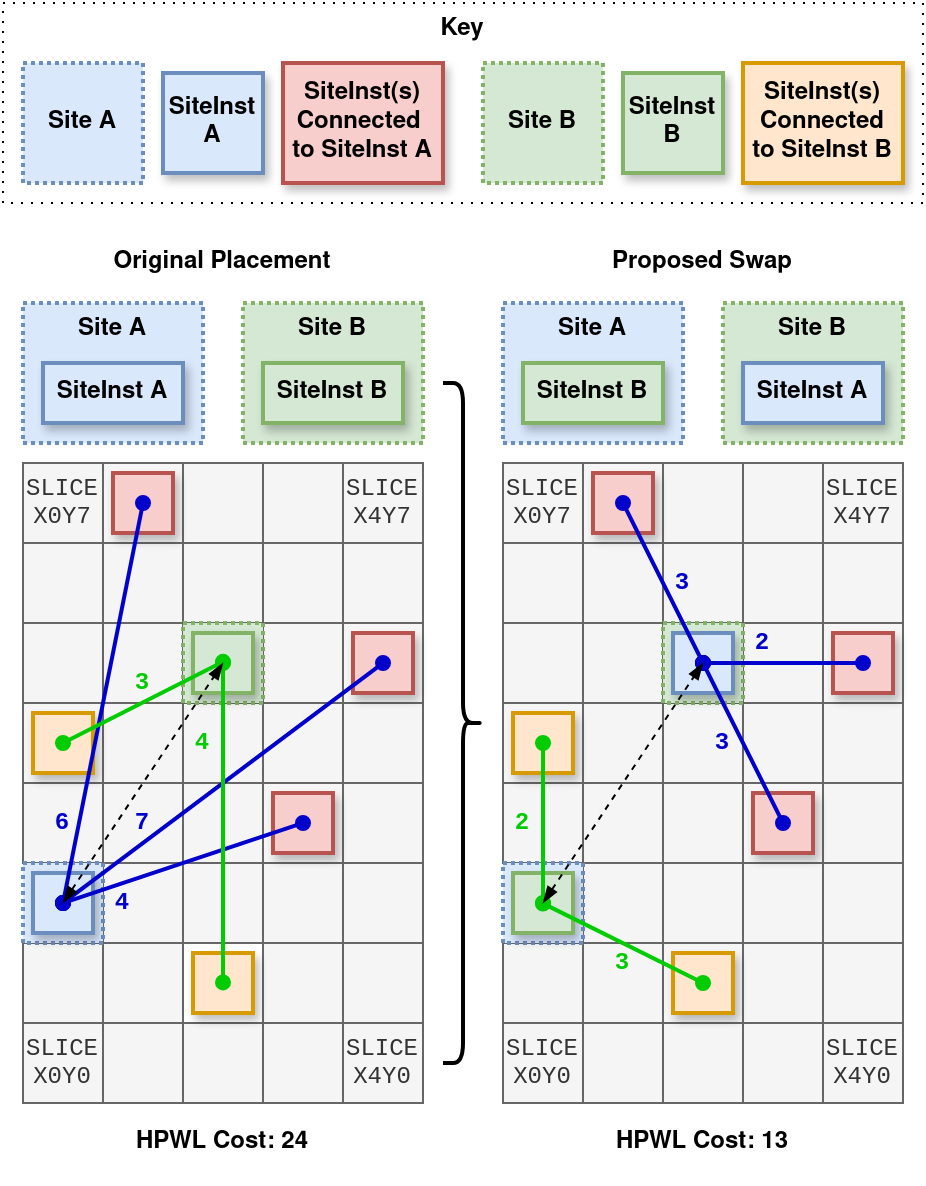
\includegraphics[width=\columnwidth]{figures/placement/swapSingleSite.png}
    \captionof{figure}{Single Site Swap Proposal}
    \label{fig:swapSingleSite}
}




